\documentclass{article}

\usepackage{ctex}
\usepackage{geometry} % 使用geometry宏包设置页面布局
\usepackage{graphicx} % 使用graphicx宏包插入图片
\usepackage{lipsum} % 使用lipsum宏包生成随机文本,用于示例
\usepackage{siunitx}
\usepackage{amsmath}
\usepackage{booktabs} % 用于制作漂亮的表格线
\usepackage{lipsum} % 示例文本
\usepackage{setspace}
\usepackage{float}
\usepackage{enumitem}
\usepackage{hyperref}
\usepackage{csvsimple} % 导入csvsimple宏包
\usepackage{multirow}
\usepackage{multicol}
\usepackage{eqnarray}
\usepackage{subfigure}
\usepackage{listings}
\usepackage{xcolor}
\newcolumntype{C}{>{$}c<{$}}


\lstdefinestyle{qtstyle}{
  language=C++, 
  backgroundcolor=\color{gray!20}, % 设置背景颜色为灰色
  basicstyle=\ttfamily\small\color{black}, % 设置基本文本为黑色
  keywordstyle=\color{blue},
  commentstyle=\color{green!40!black}, 
  stringstyle=\color{red}, 
  showstringspaces=false, 
  breaklines=true, 
  breakatwhitespace=true, 
  tabsize=4, 
  captionpos=b,
  frame=single, % 添加单线边框
  frameround=ftff, % 设置边框为矩形
  numbers=left, % 在左边添加行数
  numberstyle=\tiny\color{gray}, % 设置行数的样式
  numbersep=5pt % 设置行数与代码的间隔
}




\title{高级语言程序设计大作业实验报告}
\author{王硕 2312456 }
\date{\today}

\begin{document}

\maketitle
\tableofcontents


\section{作业题目}
\textbf{基于qt和sqlite数据库的超市管理系统}




\section{开发软件}
\textbf{Qt6.7.0 + Qt Creator 13.0.0}
\\
\indent
\textbf{Sqlite3 + Navicat Premium 16}


\section{课题要求}
\begin{itemize}[noitemsep, leftmargin=*]
\item \textbf{面向对象}
\item \textbf{数据库设计}
\end{itemize}


\section{主要内容}
\subsection{数据库设计}
这里数据库相关信息的设计是单独放在一个.h和.cpp文件中的,在设计的时候,我们首先把员工和用户的信息放入相应的结构体里面:
\begin{lstlisting}[style=qtstyle, caption={Qt代码示例}, label=qt_example]
    void Page_Login::on_btn_exit_clicked()
struct EmployInfo
{
    int id;
    QString name;
    int age;
    QString address;
    QString position;
    int salary;
};

struct UserInfo
{
   QString uername;
   QString password;
   QString auth;
};
\end{lstlisting}

之后是数据的增加,删除,更新等操作功能,相应的函数如下:(每个函数的大致功能如备注所示,具体代码见相应的sql\_manage.cpp文件)
\begin{lstlisting}[style=qtstyle, caption={Qt代码示例}, label=qt_example]
    void init();   //初始化数据库连接
    explicit sql_manage(QObject *parent = nullptr);
    
    //针对员工信息
    quint32 getCount();    //获取员工表中的员工数量
    QList<EmployInfo> getPage(quint32 page,quint32 uiCnt);  //分页查询员工信息并返回指定页码的员工信息列表
    bool add(EmployInfo);   //添加新的员工信息
    bool delEmp(int id);    //根据员工的id删除员工的信息
    void clearStuTable();   //清空员工表的数据
    void Update(EmployInfo);  //更新员工表中的数据
    QList<EmployInfo> select(QString name);   //根据员工姓名查询员工信息
    
    //针对用户账号
    QList<UserInfo> getAllUser();  //获取所有用户的信息列表
    bool isExit(QString strUser);  //检查用户的信息是否存在
    bool UpdateUser(UserInfo info);  //更新用户信息
    bool AddUser(UserInfo info);  //增加用户信息
    bool delUser(QString strUserName);  //删除用户信息
    UserInfo selUser(QString name);  //查询用户信息
\end{lstlisting}
\indent
同时通过如下代码实现了一个单例模式,确保程序中只有一个 sql\_manage 类的实例存在,并提供了静态方法 getinstance() 来获取该实例。
\begin{lstlisting}[style=qtstyle, caption={Qt代码示例}, label=qt_example]
    static sql_manage *ptrsql;
    static sql_manage *getinstance()
    {
        if(ptrsql==nullptr)
        {
            ptrsql= new sql_manage;
        }
        return ptrsql;
    }
\end{lstlisting}


\subsection{登录ui设计}
这里的ui界面主要包含两部分,分别是注册界面和登录界面。图示如下:
\\
\begin{figure}[H]
  \centering
  \subfigure[登录界面]{
    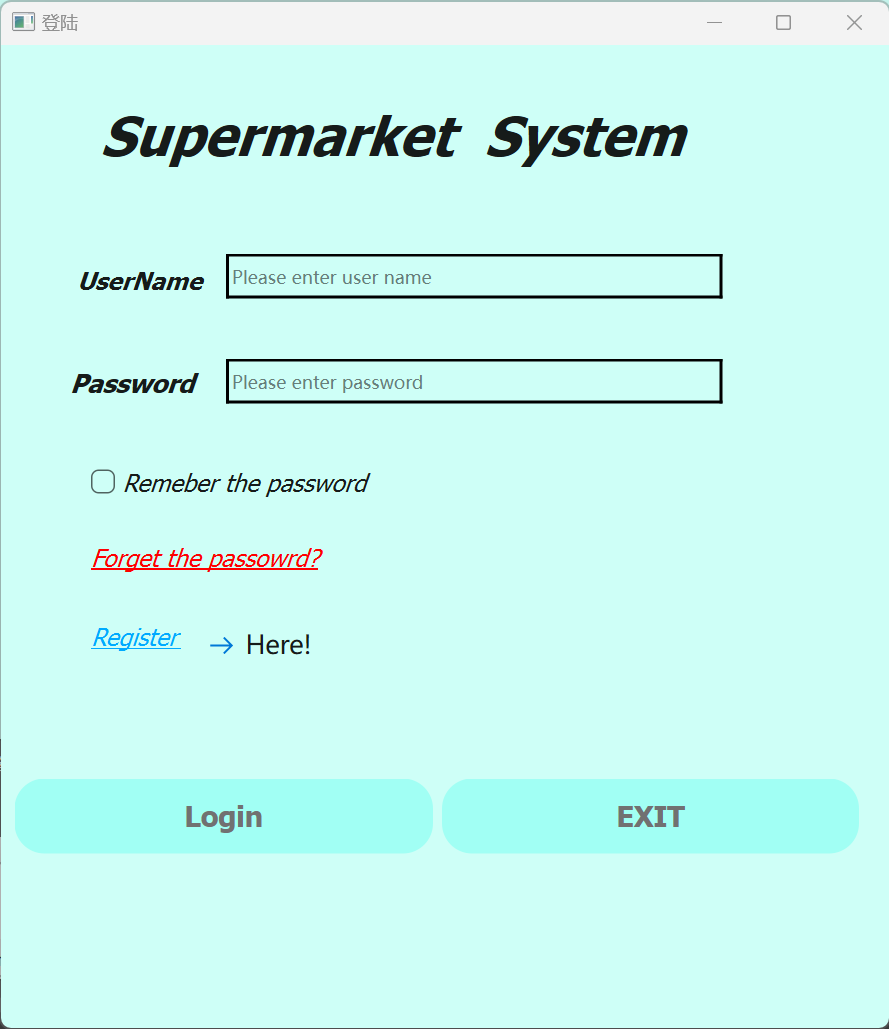
\includegraphics[width=0.45\textwidth]{登录界面.png}
    \label{fig:登录}
  }
  \hspace{0.05\textwidth} % 水平间距
  \subfigure[注册界面]{
    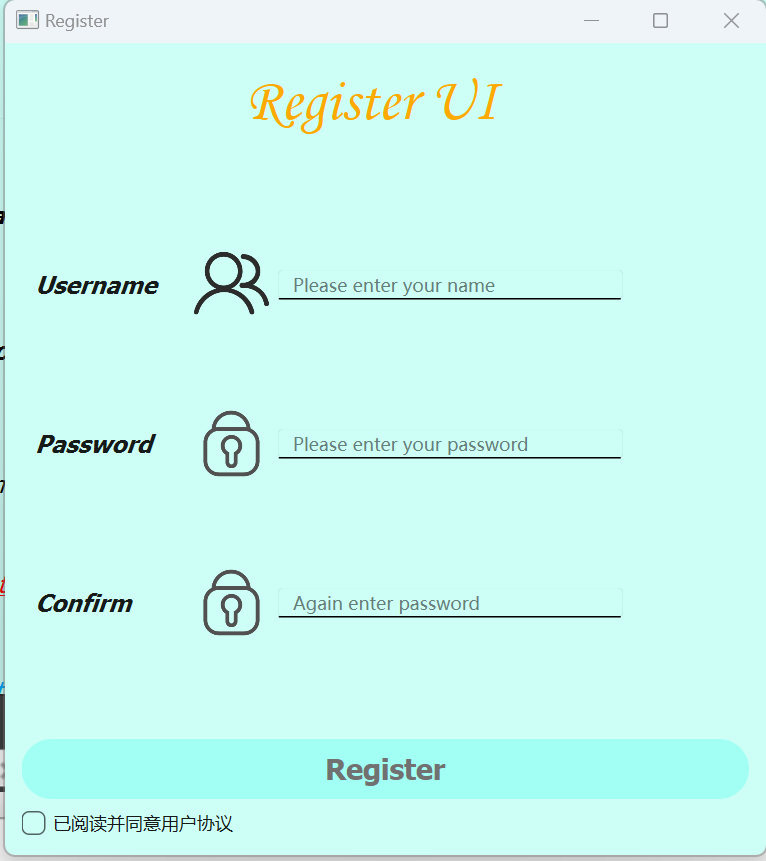
\includegraphics[width=0.45\textwidth]{注册界面.png}
    \label{fig:注册}
  }
\end{figure}
\\
\noindent
首先是界面设计的介绍,其中的字体、界面颜色等等的设计主要基于qss设计,具体代码参考相应的ui设计的代码文件,这里的排版我主要是自己手动设计的,个人感觉qt自带的界面排版设计有一点的抽象,总是设计的很习惯,后来索性我就自己一点一点的调整了(强迫症劝退),下面是一些按钮功能的介绍:
\\
\indent
\textbf{登录界面}:
\\
\noindent
关闭操作:
\begin{lstlisting}[style=qtstyle, caption={Qt代码示例}, label=qt_example]
    void Page_Login::on_btn_exit_clicked()
{
    exit(0);
}
\end{lstlisting}
\\
\noindent
登录操作:
\begin{lstlisting}[style=qtstyle, caption={Qt代码示例}, label=qt_example]
    
void Page_Login::on_btn_login_clicked()
{
    //数据库查找用户名和密码
    QString username=ui->_user->text();
    QString password=ui->password->text();
    UserInfo info= ptrUser->selUser(username);



    //失败就提示 成功进入主界面
        if(info.uername==username&&info.password==password)
        {

            QMessageBox::information(this, tr("Sucess!"),  tr("登陆成功!"),
                                                     QMessageBox::Ok);
            this->hide();
            emit sendLoginSucess();
        }
        else
        {
            QMessageBox::warning(this, tr("危险弹窗"),  tr("警告!!!\n密码或用户名错误!\n请重新输入!"),
                                                     QMessageBox::Ok);
            ui->_user->clear();
            ui->password->clear();
        }


}
\end{lstlisting}
\\
\noindent
进入注册界面的操作:
\begin{lstlisting}[style=qtstyle, caption={Qt代码示例}, label=qt_example]
    void Page_Login::on_commandLinkButton_clicked()
{
    reg.show();
    this->hide();


    auto f= [&](){
        this->show();
    };

    connect(&reg,&page_register::sendRegisterSucess,this,f);

}

\end{lstlisting}


\\
\indent
\textbf{注册界面}:
\\
\noindent
注册操作:
\begin{lstlisting}[style=qtstyle, caption={Qt代码示例}, label=qt_example]
    void page_register::on_registerButton_clicked()
{
    UserInfo info=getinfo();
    if(info.uername.isEmpty())
    {
        QMessageBox::warning(this, tr("危险弹窗"),  tr("警告!!!\n两次输入密码不同!"),
                                        QMessageBox::Ok);
        ui->passwordLineEdit->clear();
        ui->confirmLineEdit->clear();
    }
    else
    {
        ptrsql->AddUser(info);

       this->hide();
       emit sendRegisterSucess();
    }

}
\end{lstlisting}
\\
\indent
剩下的关于label和text的设计就不在过多描述。

\subsection{管理ui设计}
首先是主界面的设计,相应的展示图如下:
\begin{figure}[H]
        \centering
        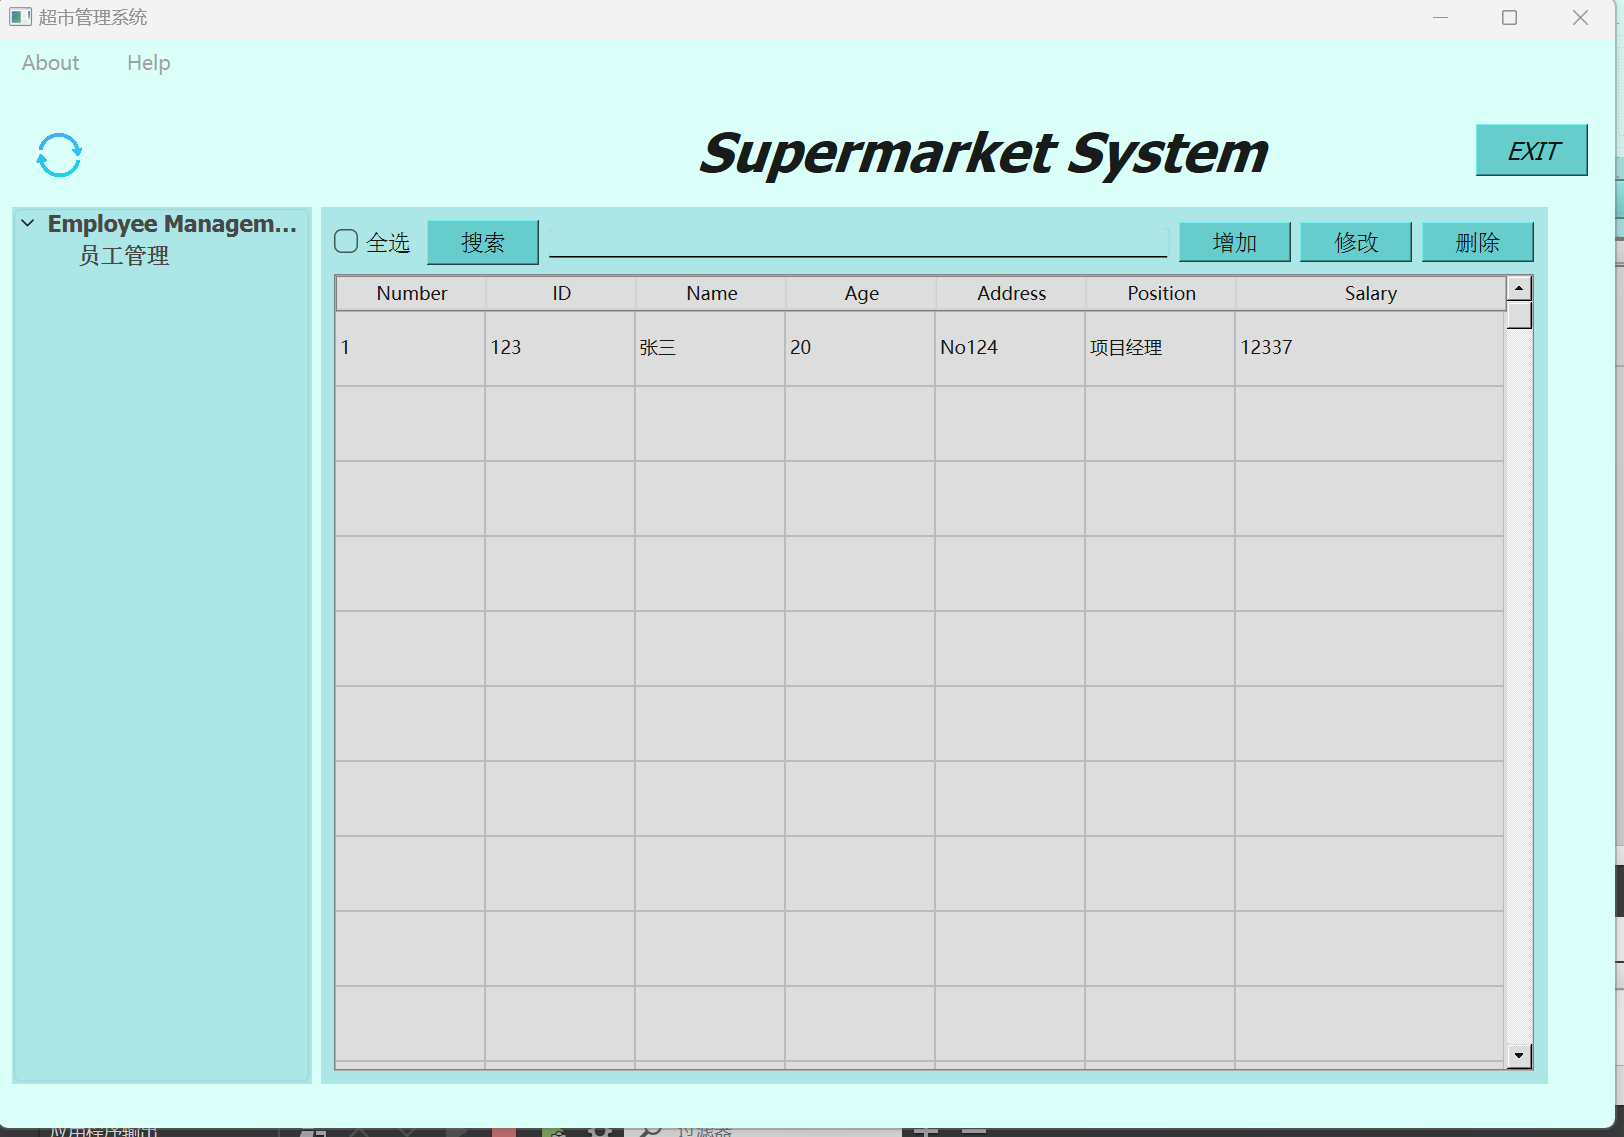
\includegraphics[scale=0.6]{主界面.png}
        \caption{主界面示意图}
        \label{fig:enter-label}
\end{figure}
整体来说,这个主界面首先使用了一个QGridLayout的布局管理系,将主窗口分成左右两个部分,之后在左侧放置了一个QTreeWidget控件用于显示树状结构的数据,右侧放置了一个QStackedWidget控件,用与显示多个页面,可以根据需要切换显示不同的页面。之后就是一些常规的按钮,比如增加,修改,删除等等的按钮,还有相应的itemform插入在界面中,用于显示用户的信息。按钮的功能就不在这里一一描述,参考相应的mainwindows.cpp和itemform.cpp文件。
\\
下面是一些按钮功能的介绍:
\begin{lstlisting}[style=qtstyle, caption={Qt代码示例}, label=qt_example]
    void on_deleteButton_clicked();  //删除员工信息

    void on_updateButton_clicked();  //更新员工信息

    void on_addButton_clicked();  //添加员工信息

    void on_exitButton_clicked(); //退出界面
    
    void showList();  //从数据库中获取员工信息并在表格中显示出来

    void on_searchButton_clicked();  //查询员工信息

    void on_showButton_clicked();  //重新加载并显示员工信息

\end{lstlisting}
\\
除此之外就是一个小小的一个增添信息的界面,如下图所示:
\begin{figure}[H]
        \centering
        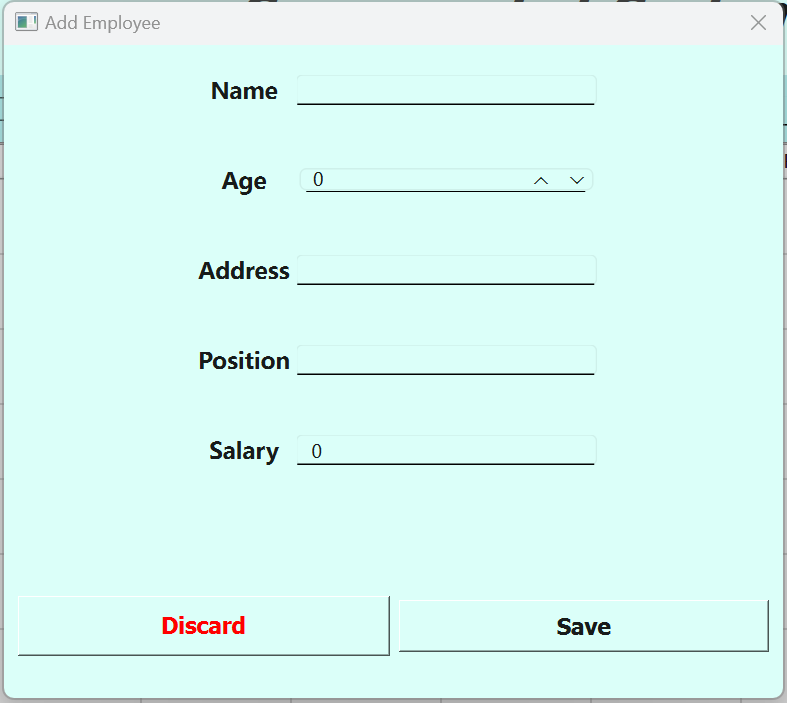
\includegraphics[scale=0.6]{输入界面.png}
        \caption{增添信息界面示意图}
        \label{fig:enter-label}
\end{figure}
其具体的功能参考相应的addempdialog.cpp文件。



\section{收获、思考以及我的创作历程}
总体来说,其实这次做c++大作业收获是多的,我也是第一次接触到数据库,当时想做这个的初衷也是想要学习新的知识,可能表现能力比较差吧,没有什么特效,不过总体来说还可以,能收获到很多也很不错。近几年我看很多人都在做游戏,我就在想能不能换一个思路,做一个比较有实际的东西(主要是游戏的话网上也有很多源代码,而且游戏的题材大多雷同,所以就不太想做),之后在跟高中同学聊天的过程中他跟我提到了这个,于是我就想这个能不能尝试做出来这个,但很显然最终的结果算是失败的吧,只能是说做出来一个残次品出来,最终我也没能把数据库和qt连接起来(不知道是不是我的电脑的问题,等到我想要换个题材做的时候也已经没有时间了)。开始的时候我用的是mysql,但是我的qt总是显示没有相关mysql驱动器(刚开始我连问题都没发现,大概找了一下午才知道自己的问题大致在哪里),之后我就开始去着手解决这个问题,按照网上的教程把相应的mysql.lib和另外一个(名字忘了)文件放在qt的bin目录中,但还是失败,之后又是一段痛苦的搜查问题的过程,然后就知道了qt的6.0以上的版本是不自带mysql的sqldriver文件的,而且要自己写......,可以想象一下我此时的精神状态,好在我没有一股脑写下去,去网上搜了一下发现有的github的大佬已经写好了,于是就是下载,给qt增添文件的过程,结果一顿操作下来还是不行....后面好像是意识到版本不匹配的问题,于是我就把mysql的给删了,打算重新下载,结果密码总是不对....当时我就崩了,想了想就算了,于是把数据库换成了sqlite了,但是后面的结果也是类似的,qt自带sqlite的qsqldriver文件的,但到最后我还是没有成功的连接,只能是展示成这样了,不过后边我打算自学一段时间数据库,然后再去完善一下这个超市管理系统吧,感觉这个都快变成我心中的噩梦了。

\section{后面的设想}
当时由于数据库的连接问题,把整个员工的信息全部记录之后就没再往下写了,其实还有相应的货物管理,参考了一下网上的一些博主做的,找了一个不错的(如下图):
\begin{figure}[H]
        \centering
        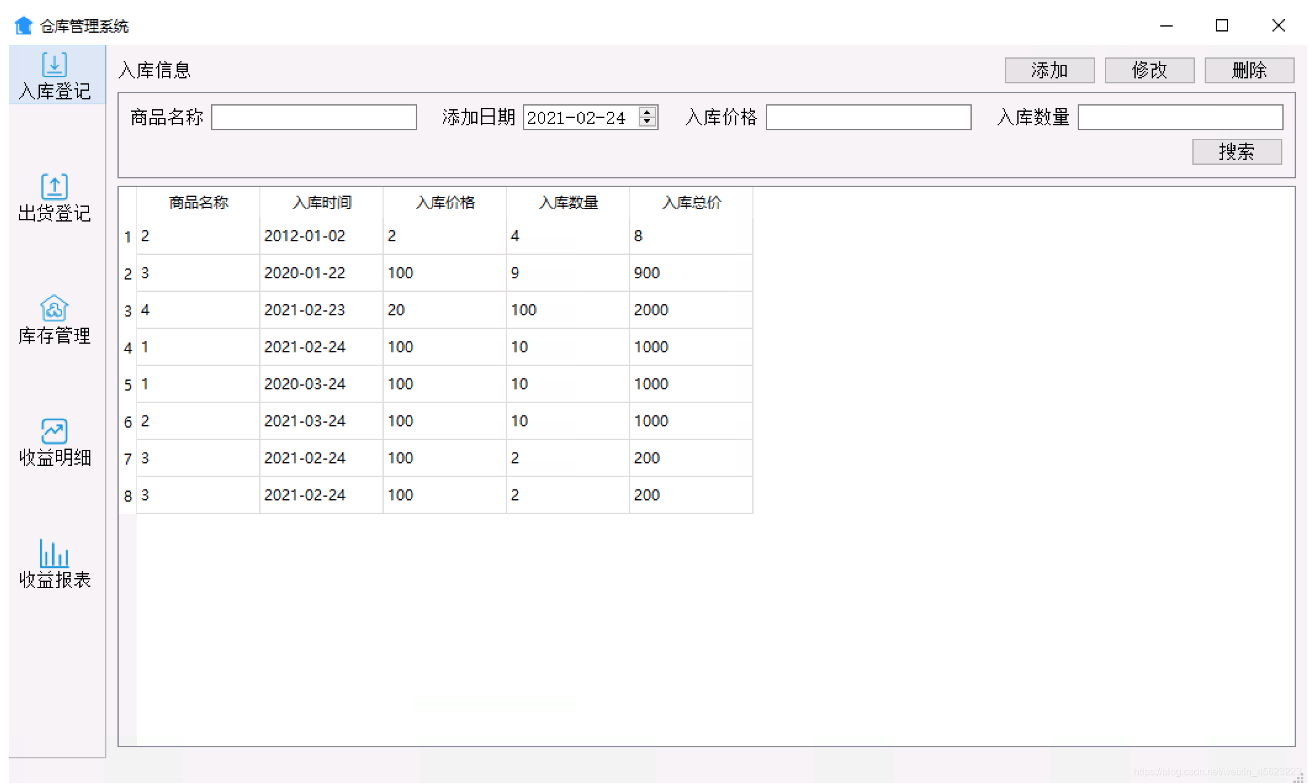
\includegraphics[scale=0.6]{设想.png}
        \label{fig:enter-label}
\end{figure}
其实当时就想做这个...数据库我都在navicate里面设计好了,发现不能用(苦笑)(我当时甚至还画出了相应的思维导图...)。之后再尝试着实现吧。
\begin{figure}[H]
        \centering
        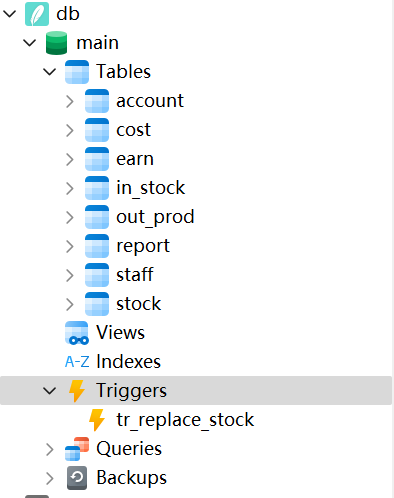
\includegraphics[scale=0.6]{数据库.png}
        \label{fig:enter-label}
\end{figure}
\begin{figure}[H]
        \centering
        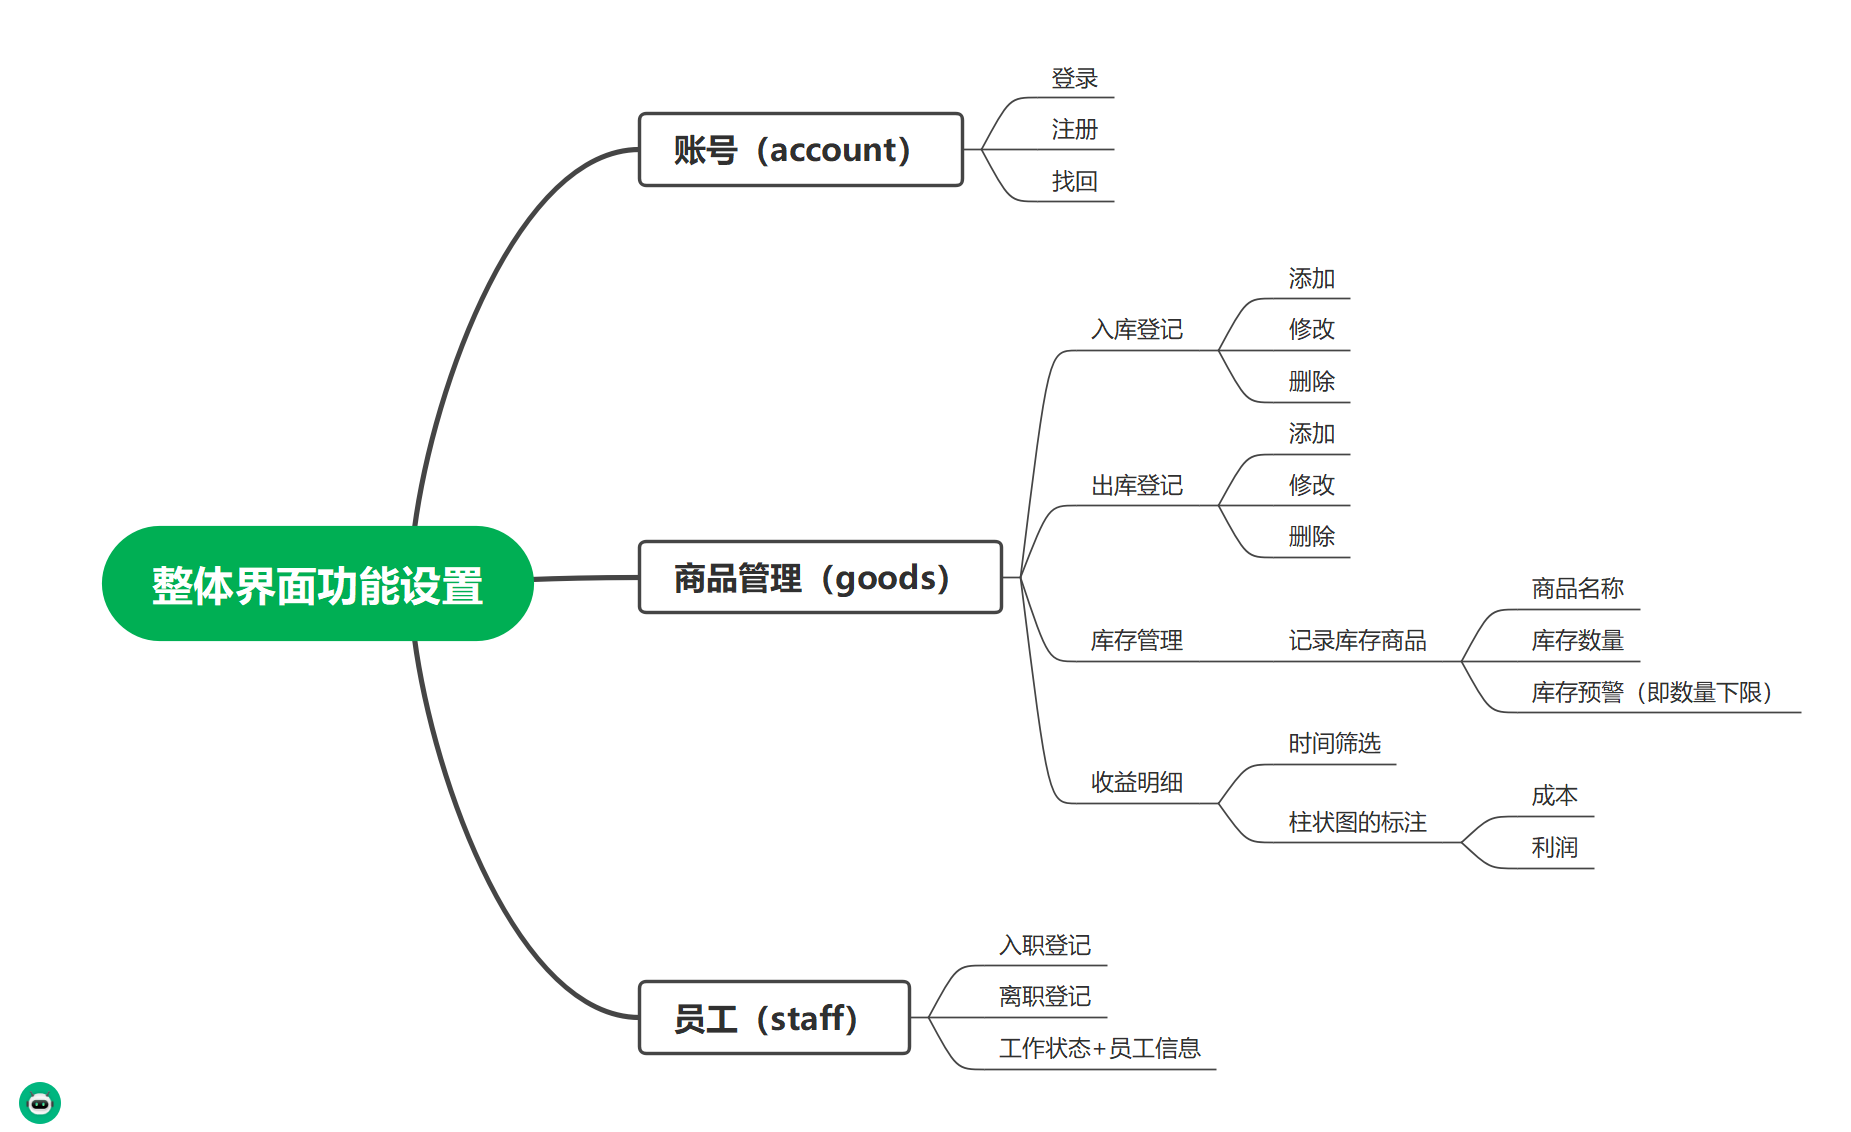
\includegraphics[scale=0.6]{1.png}
        \label{fig:enter-label}
\end{figure}
\begin{figure}[H]
        \centering
        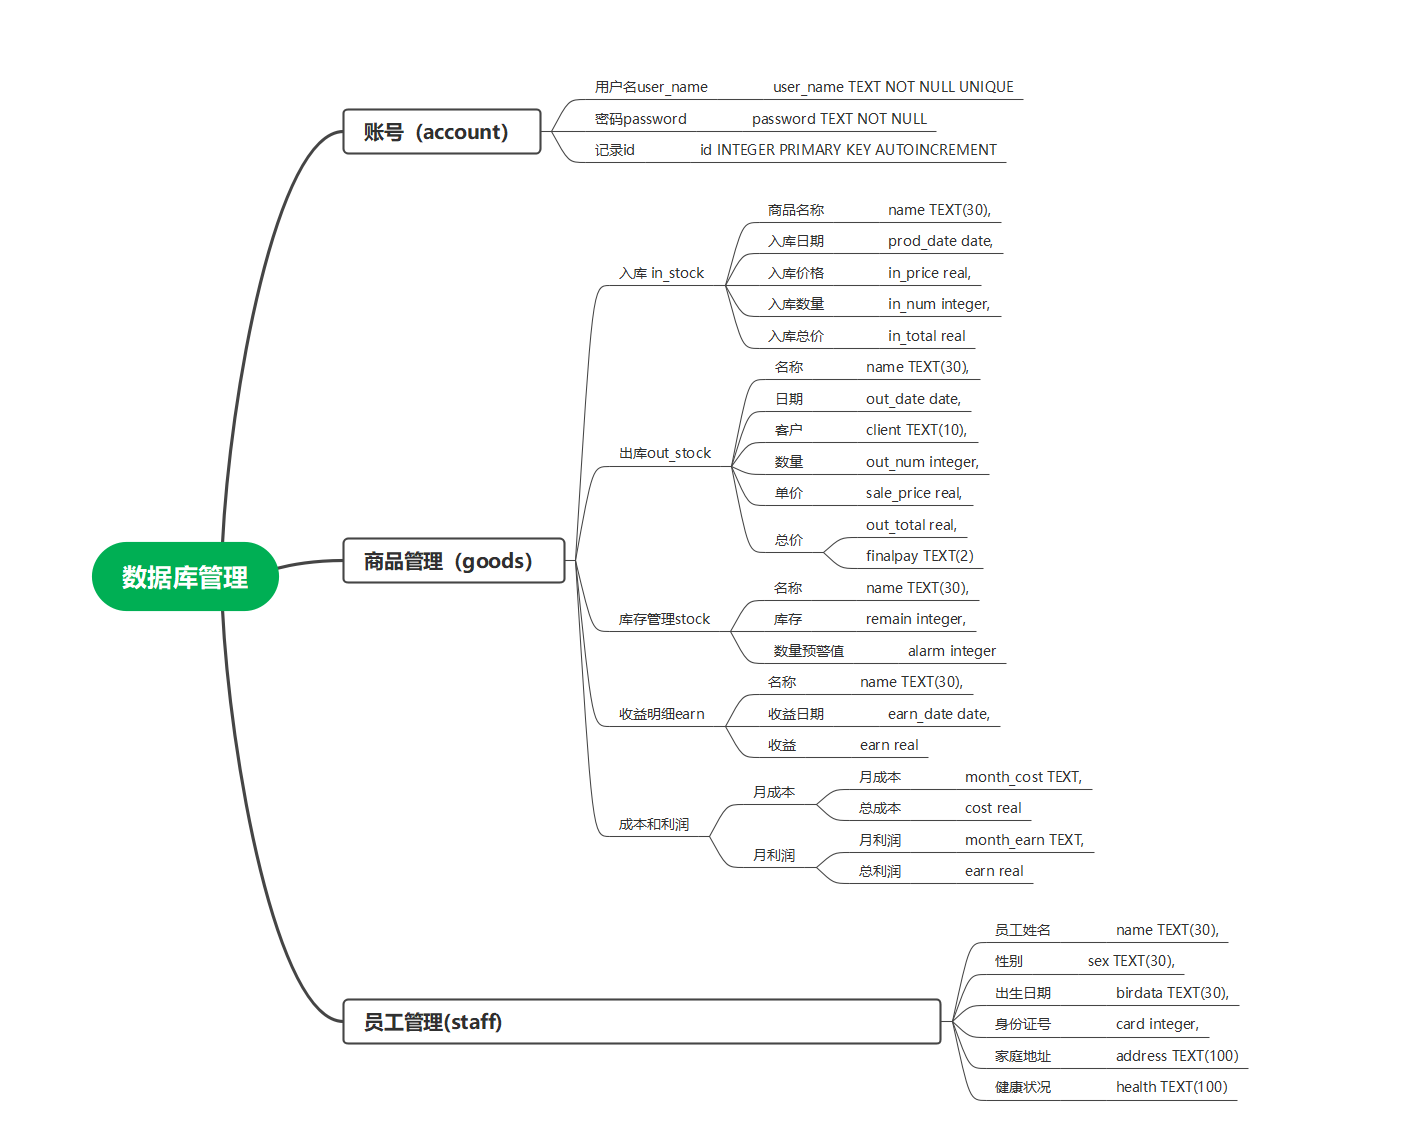
\includegraphics[scale=0.6]{2.png}
        \label{fig:enter-label}
\end{figure}

\end{document}
